\chapter{Testing and Evaluation}
\label{chap:testing-evaluation}

\section{Testing Strategy}
\label{sec:testing-strategy}

The evaluation compares real and synthetic datasets under matched experimental conditions. The testing strategy combines:
\begin{itemize}
  \item \textbf{visual diagnostics} through PCA \cite{jolliffe2002} and t-SNE \cite{vandermaaten2008};
  \item \textbf{cluster-number recovery} through success-rate analysis; and
  \item \textbf{structural diagnostics} through Gini, Mean Centroid Distance, and Mean Variance Difference.
\end{itemize}

This layered strategy is important because cluster-number recovery alone cannot reveal whether an apparently correct solution still distorts the original geometry.

\section{Visual Evaluation}
\label{sec:visual-evaluation}

\subsection{Principal Component Analysis}
Principal Component Analysis (PCA) preserves global linear structure and is therefore useful for identifying large-scale distortions introduced by decision-tree synthesis \cite{jolliffe2002}. In the figures below, the intended reading order is the same in both distributions: top row for real data, bottom row for synthetic data, with true labels on the left and clustering outputs in the center and right panels.

\subsubsection{Normal Distribution}
\begin{figure}[H]
  \centering
  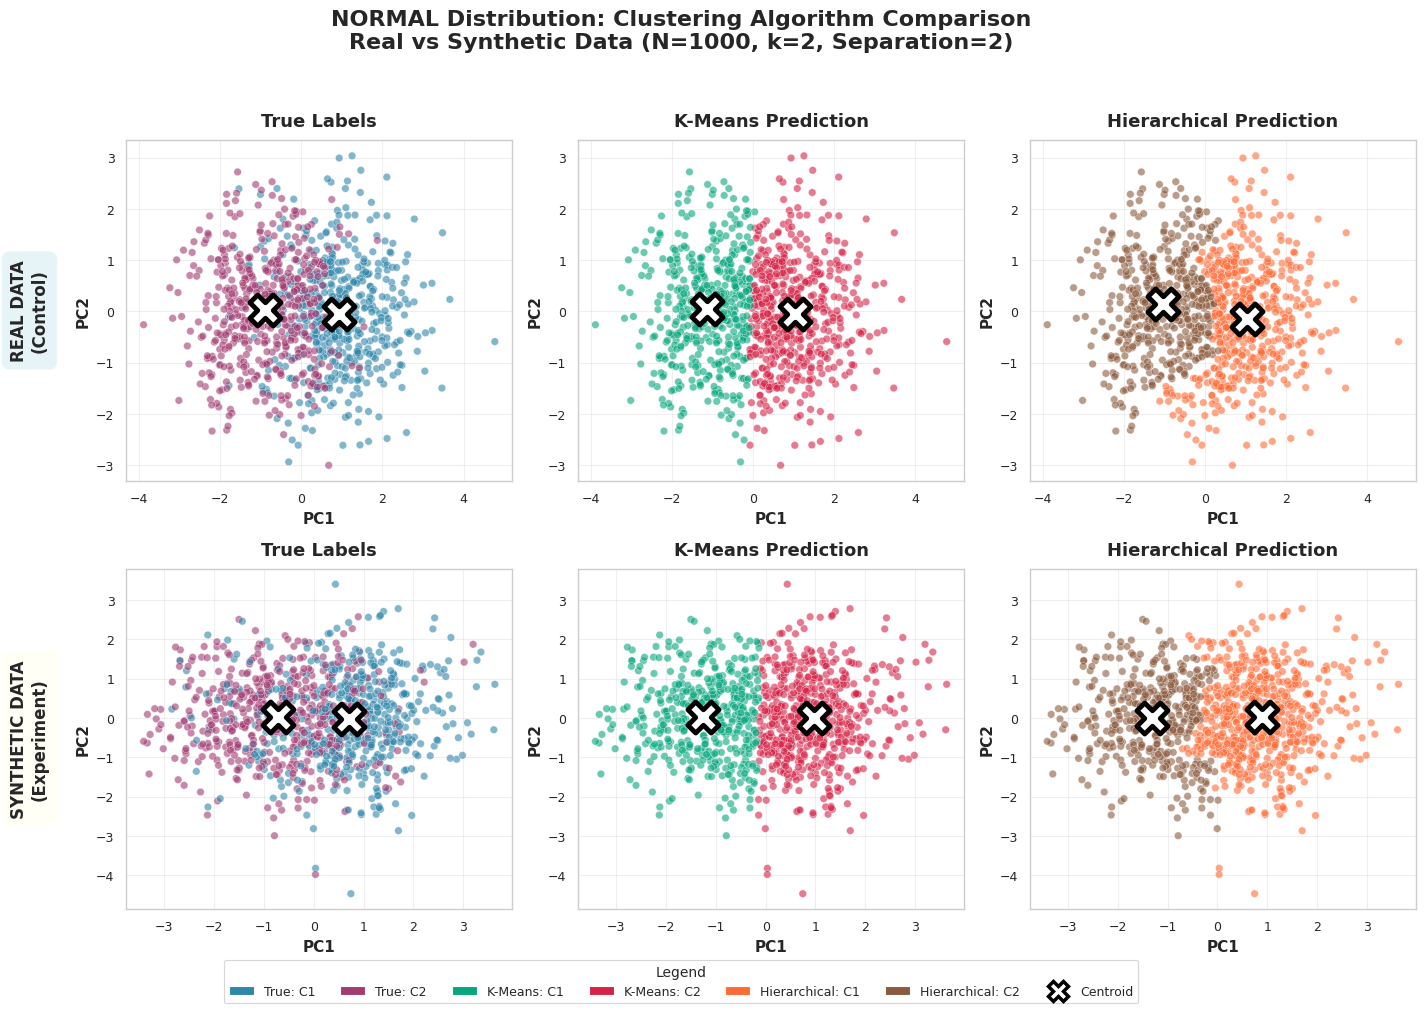
\includegraphics[width=0.9\linewidth]{images/normal_pca.png}
  \caption{\textbf{PCA Projection: Normal Distribution ($N=1000, k=2$).} Comparison of real (top) versus synthetic (bottom) data, with true labels (left), k-means partitions (center), and hierarchical-clustering partitions (right).}
  \label{fig:pca_normal}
  \source{Compiled by the author}
\end{figure}

For normally distributed data, the synthetic clusters remain close to the spherical geometry of the real reference set. Both K-Means and Hierarchical Clustering recover the structure successfully, which indicates that CART synthesis is sufficiently faithful in this setting.

\subsubsection{Gamma Distribution}
\begin{figure}[H]
  \centering
  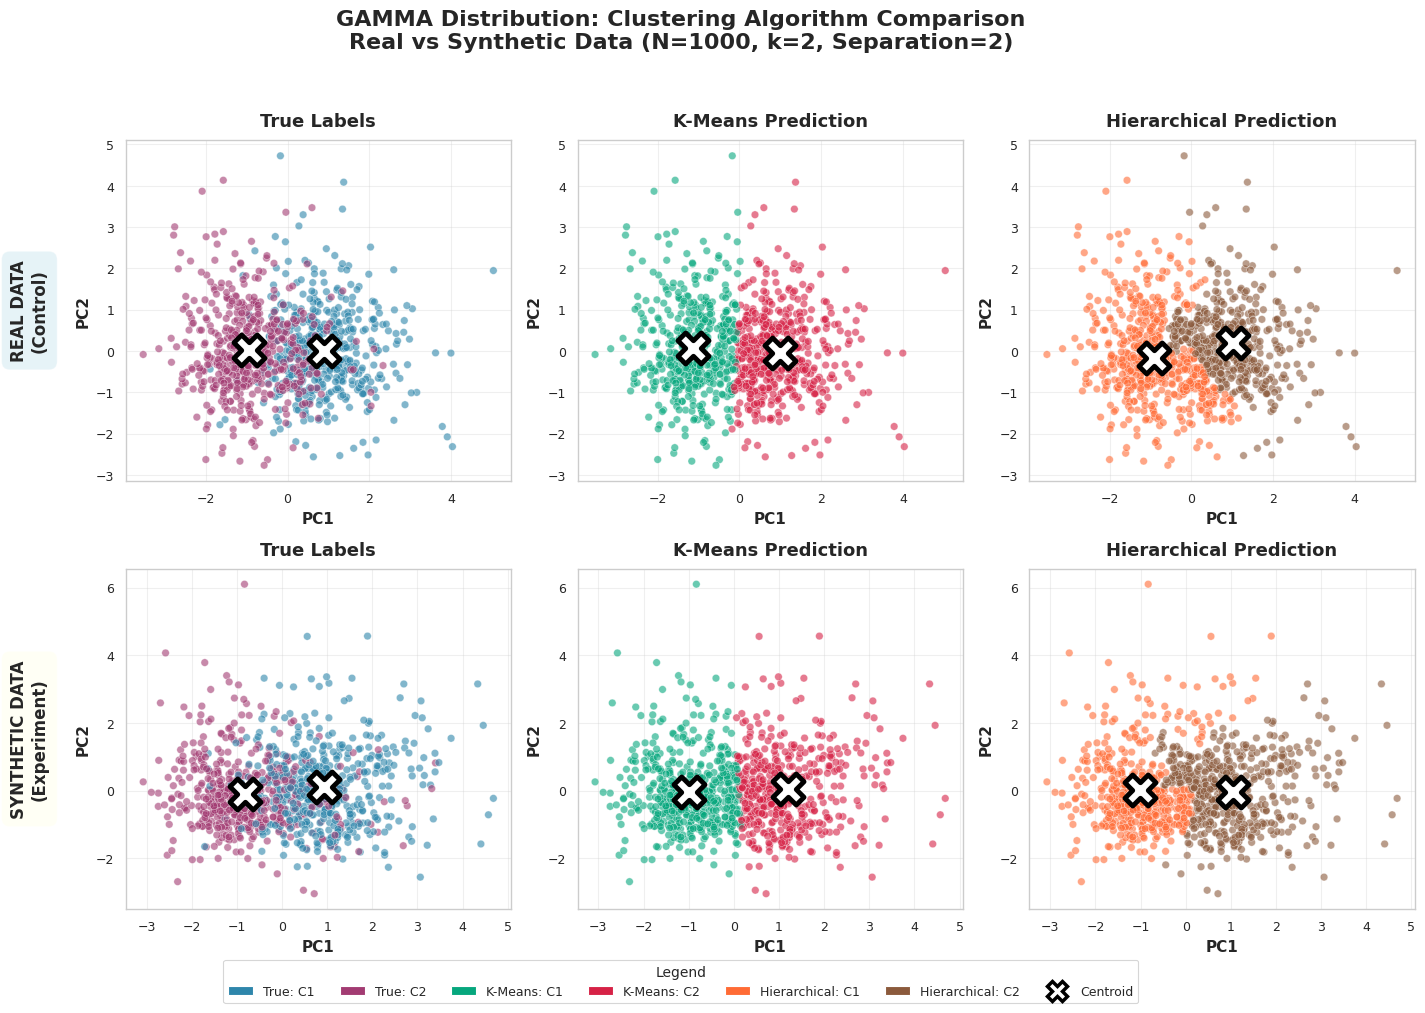
\includegraphics[width=1\linewidth]{images/gamma_pca.png}
  \caption{\textbf{PCA Projection: Gamma Distribution ($N=1000, k=2$).} Comparison of real (top) versus synthetic (bottom) data, with true labels (left), k-means partitions (center), and hierarchical-clustering partitions (right).}
  \label{fig:pca_gamma}
  \source{Compiled by the author}
\end{figure}

For gamma-distributed data, the synthetic version exhibits visibly sharper and more axis-aligned boundaries than the real reference data. These distortions are particularly problematic for k-means, which imposes rigid centroid-based partitions on geometry that is no longer well approximated by convex clusters. Hierarchical Clustering remains closer to the original structure.

\subsection{t-SNE Analysis}
t-SNE provides a non-linear view of the multidimensional data and helps reveal local separation patterns that may remain hidden under linear projection \cite{vandermaaten2008}.

\subsubsection{Normal Distribution}
\begin{figure}[H]
  \centering
  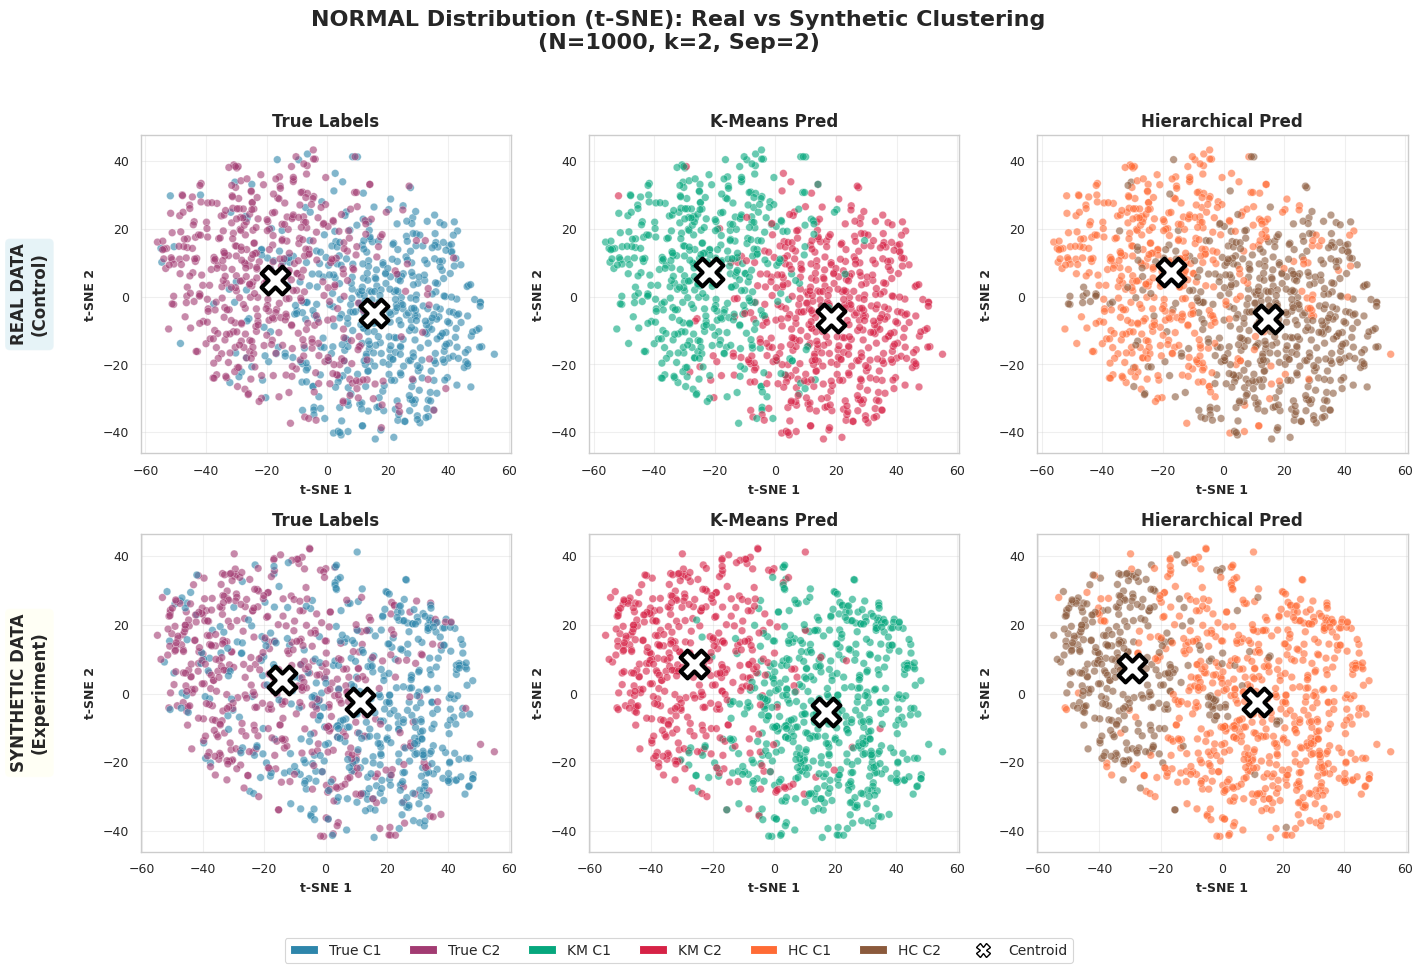
\includegraphics[width=1\linewidth]{images/normal_tsne.png}
  \caption{\textbf{t-SNE Projection: Normal Distribution.} Comparison of real (top) versus synthetic (bottom) data, with true labels (left), k-means partitions (center), and hierarchical-clustering partitions (right).}
  \label{fig:tsne_normal}
  \source{Compiled by the author}
\end{figure}

The normal case remains cohesive and well separated after synthesis. Both clustering algorithms produce nearly identical partitions, confirming that synthetic-data utility is high for spherical distributions.

\subsubsection{Gamma Distribution}
\begin{figure}[H]
  \centering
  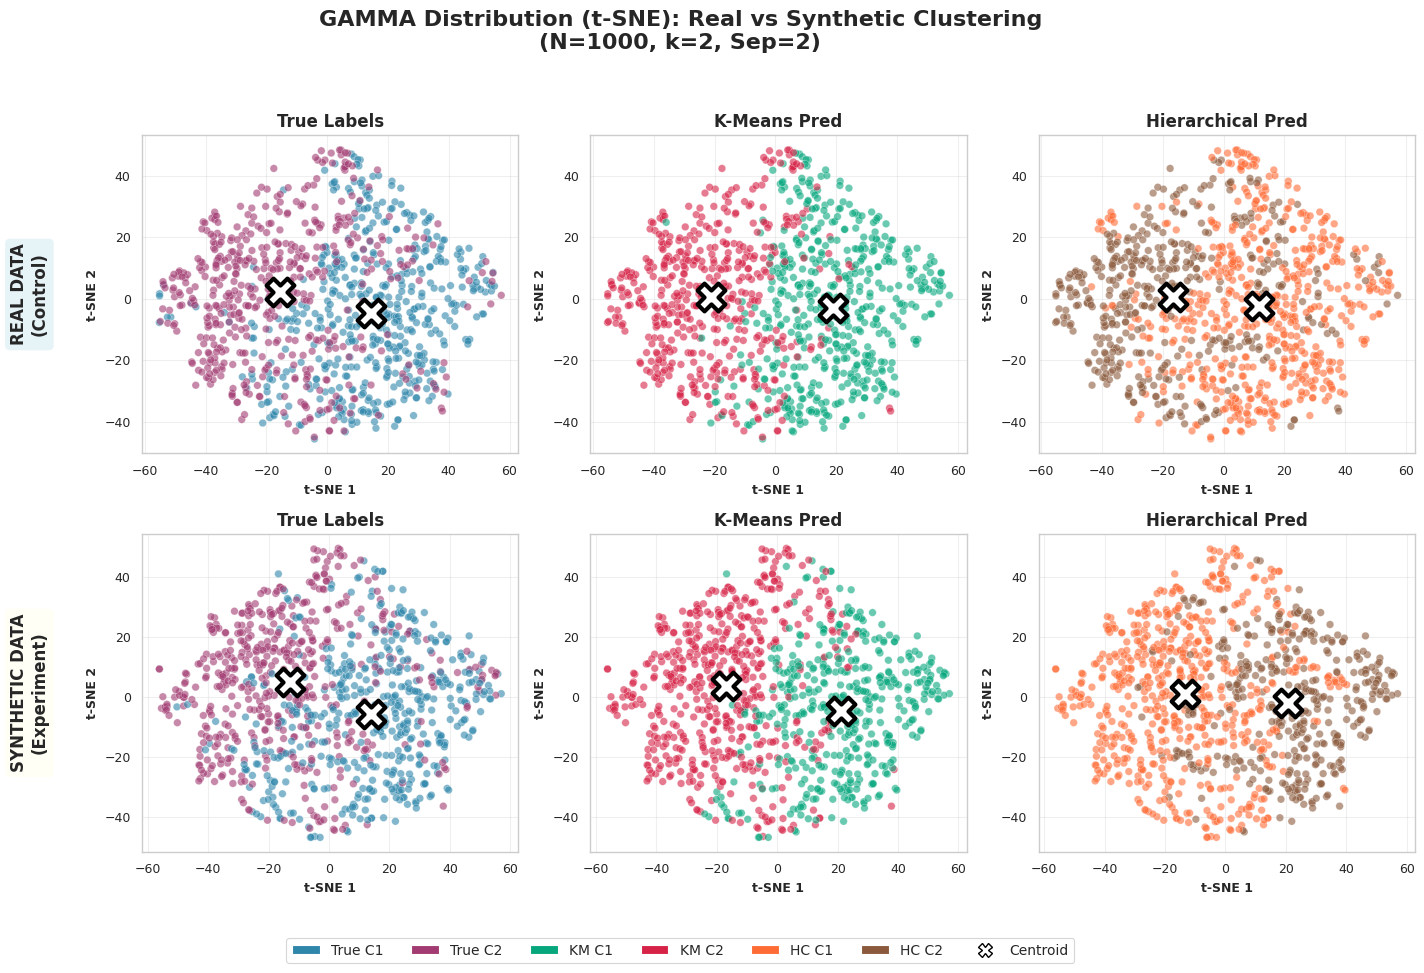
\includegraphics[width=1\linewidth]{images/gamma_tsne.png}
  \caption{\textbf{t-SNE Projection: Gamma Distribution.} Comparison of real (top) versus synthetic (bottom) data, with true labels (left), k-means partitions (center), and hierarchical-clustering partitions (right).}
  \label{fig:tsne_gamma}
  \source{Compiled by the author}
\end{figure}

The gamma case exposes the central failure mode of K-Means. On the synthetic data, K-Means slices connected density regions with rigid decision boundaries, while Hierarchical Clustering follows the connected structures more naturally.

\section{Cluster-Number Recovery}
\label{sec:cluster-number-recovery}

\subsection*{Normal Distribution}
\begin{figure}[H]
  \centering
  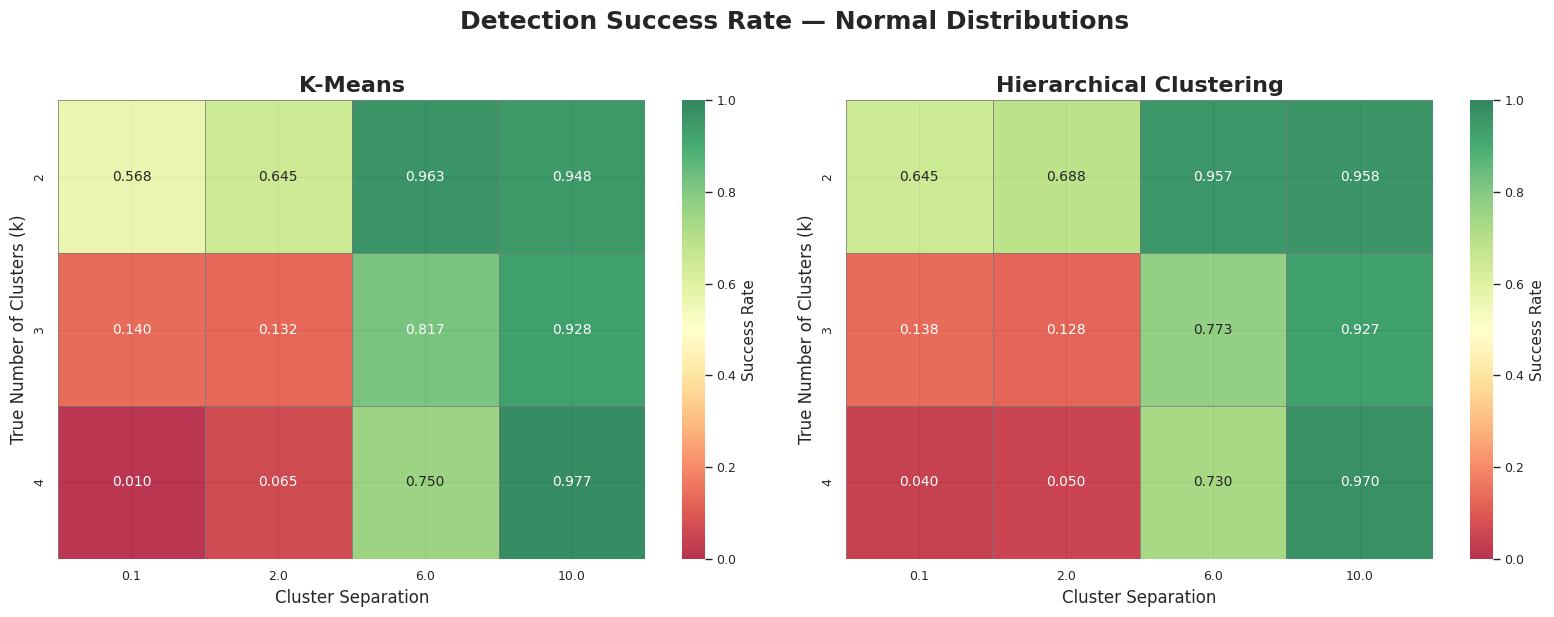
\includegraphics[width=1\linewidth]{images/dsr_normal.png}
  \caption{\textbf{Success Rate on Normal Distribution.} Left: K-Means. Right: Hierarchical Clustering.}
  \label{fig:success_normal}
  \source{Compiled by the author}
\end{figure}

For well-separated normal clusters, both algorithms achieve near-perfect recovery. Performance degrades sharply only when separation is very low, which suggests that in spherical overlapping settings the synthesis artifacts affect both methods similarly.

\subsection*{Gamma Distribution}
\begin{figure}[H]
  \centering
  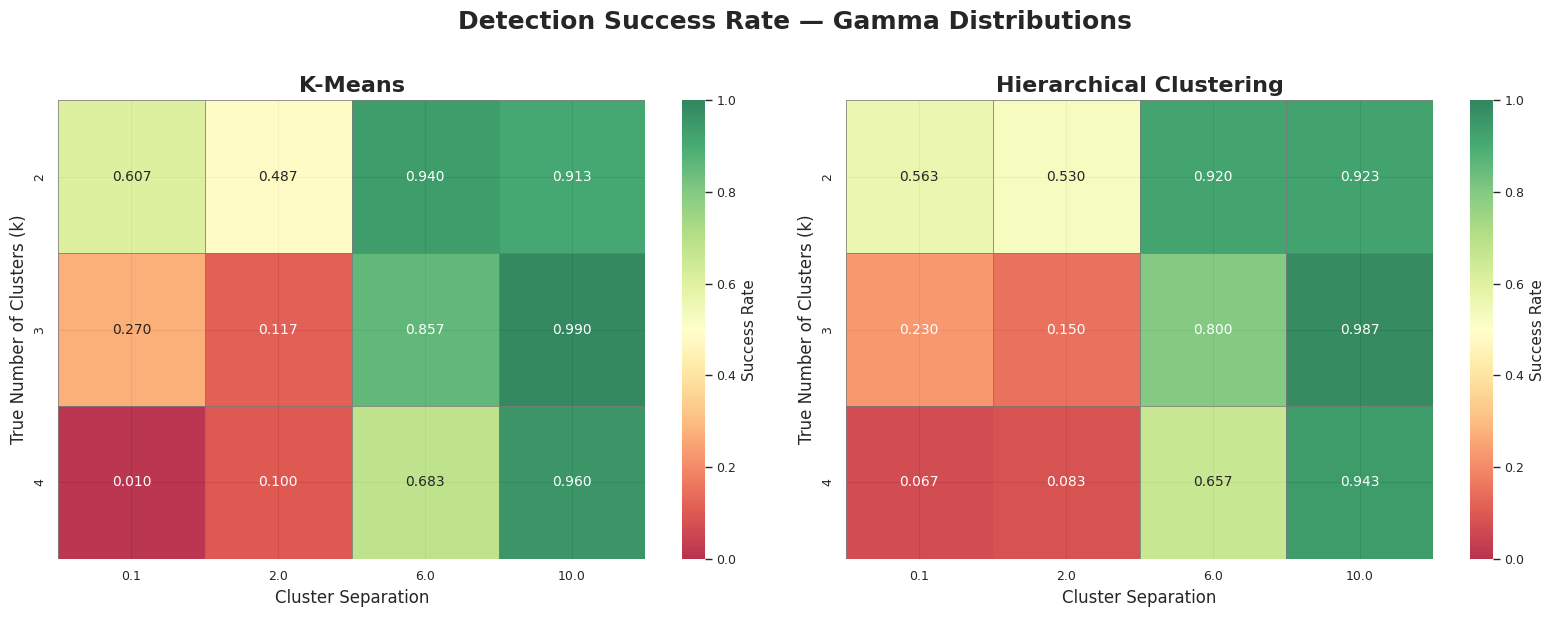
\includegraphics[width=1\linewidth]{images/dsr_gamma.png}
  \caption{\textbf{Success Rate on Gamma Distribution.} Left: K-Means. Right: Hierarchical Clustering.}
  \label{fig:success_gamma}
  \source{Compiled by the author}
\end{figure}

The gamma experiments show a clear divergence. K-Means collapses across a larger region of the parameter space, especially in moderate-separation scenarios, whereas Hierarchical Clustering retains substantially higher recovery rates. This is the first strong empirical signal that connectivity-based clustering is more robust to the synthetic distortions introduced by CART.

\section{Structural Fidelity Metrics}
\label{sec:structural-fidelity}

\subsection{Gini Coefficient}
\begin{figure}[H]
  \centering
  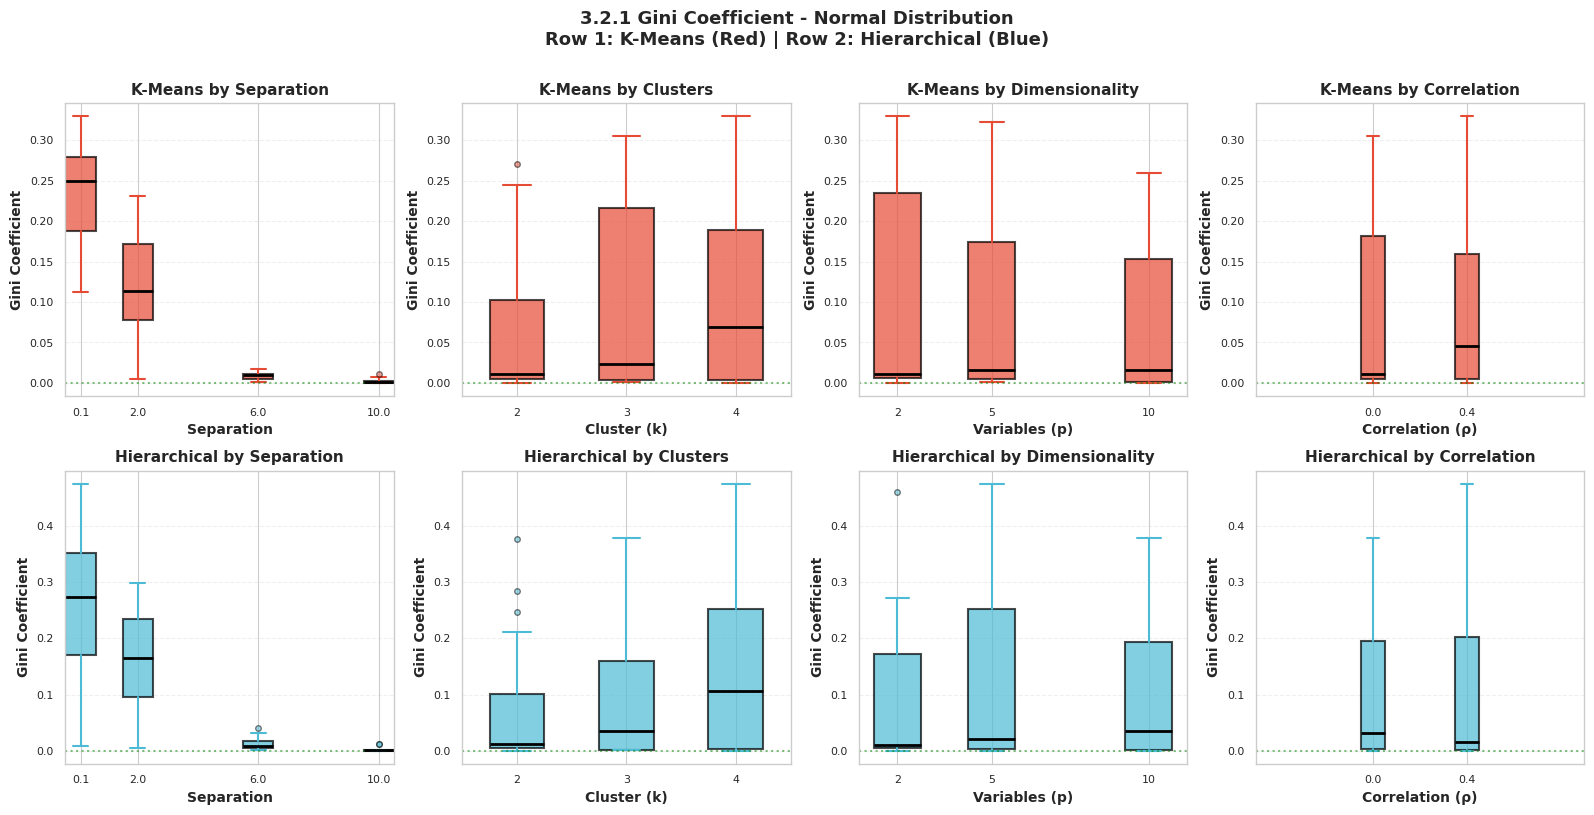
\includegraphics[width=\textwidth]{images/gini_normal.png}
  \caption{\textbf{Absolute Gini Coefficients (Normal Distribution).} Row 1: K-Means. Row 2: Hierarchical Clustering.}
  \label{fig:gini_absolute_normal}
  \source{Compiled by the author}
\end{figure}

\begin{figure}[H]
  \centering
  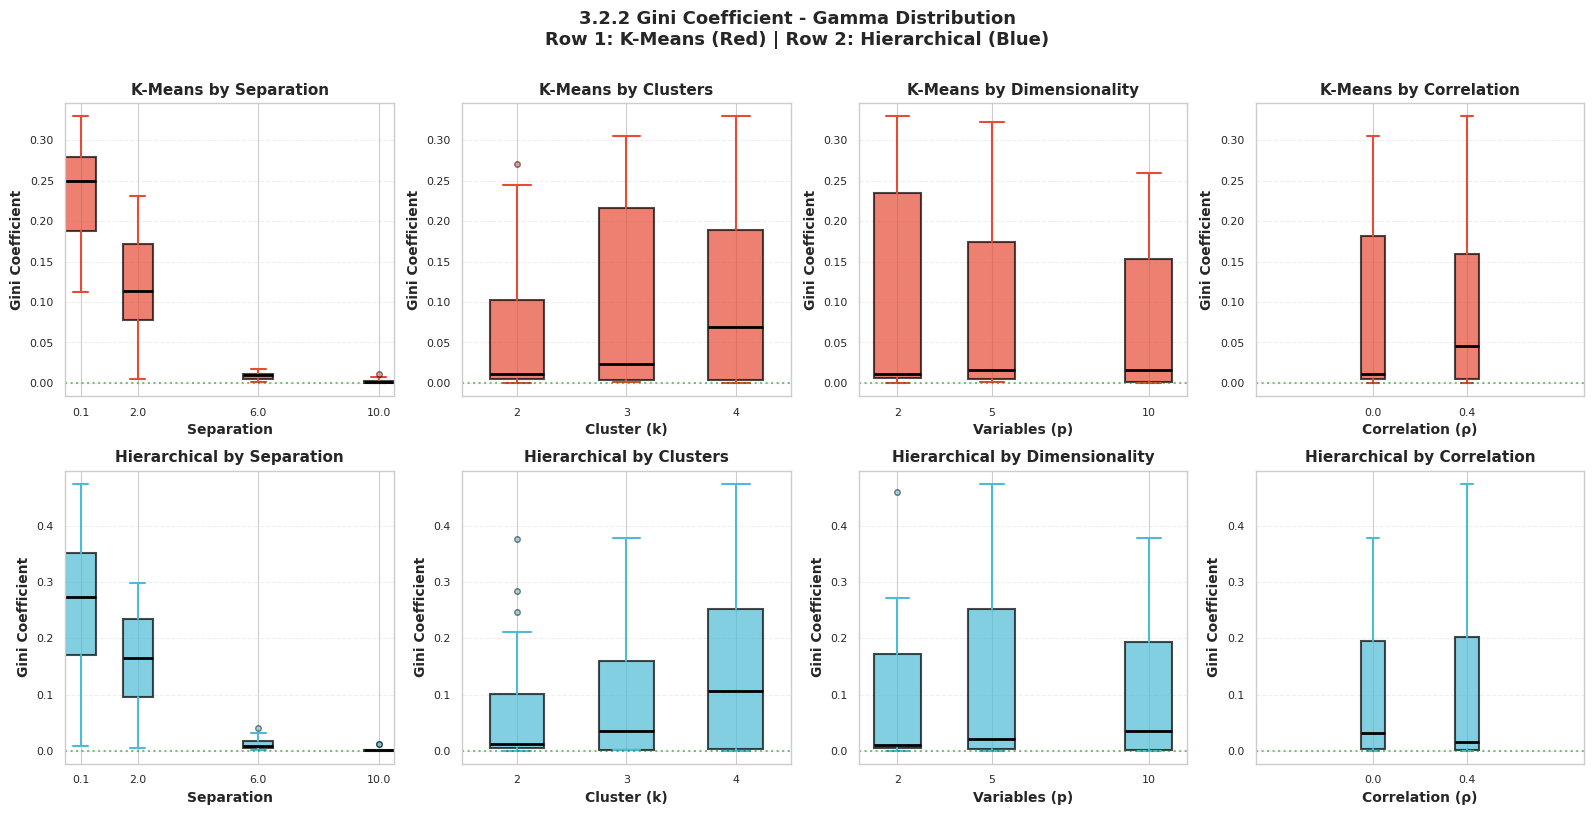
\includegraphics[width=\textwidth]{images/gini_gamma.png}
  \caption{\textbf{Absolute Gini Coefficients (Gamma Distribution).} Row 1: K-Means. Row 2: Hierarchical Clustering.}
  \label{fig:gini_absolute_gamma}
  \source{Compiled by the author}
\end{figure}

Chapter~\ref{sec:evaluation-metrics} defines fidelity in terms of the \emph{difference} between the Gini index of the real-data partition and that of the synthetic-data partition, $\Delta G = |G^{(R)} - G^{(S)}|$. The figures available in the review package, however, report absolute Gini values for the clustering outputs rather than a dedicated $\Delta G$ panel. For that reason, the discussion here is descriptive rather than definitive: the plots characterize how balanced the partitions are, but they do not by themselves prove fidelity or bias unless the real-data baseline is shown explicitly.

Within that limitation, the normal regime shows that both algorithms converge toward balanced partitions as separation increases. In the gamma regime, k-means tends to produce low-Gini partitions even when the underlying geometry is skewed, whereas Hierarchical Clustering allows more imbalance and higher variability. This pattern is consistent with the idea that k-means smooths the data geometry more aggressively, but the absolute plots alone are not sufficient to quantify that effect as a fidelity score.

\subsection{Mean Centroid Distance}
\begin{figure}[H]
  \centering
  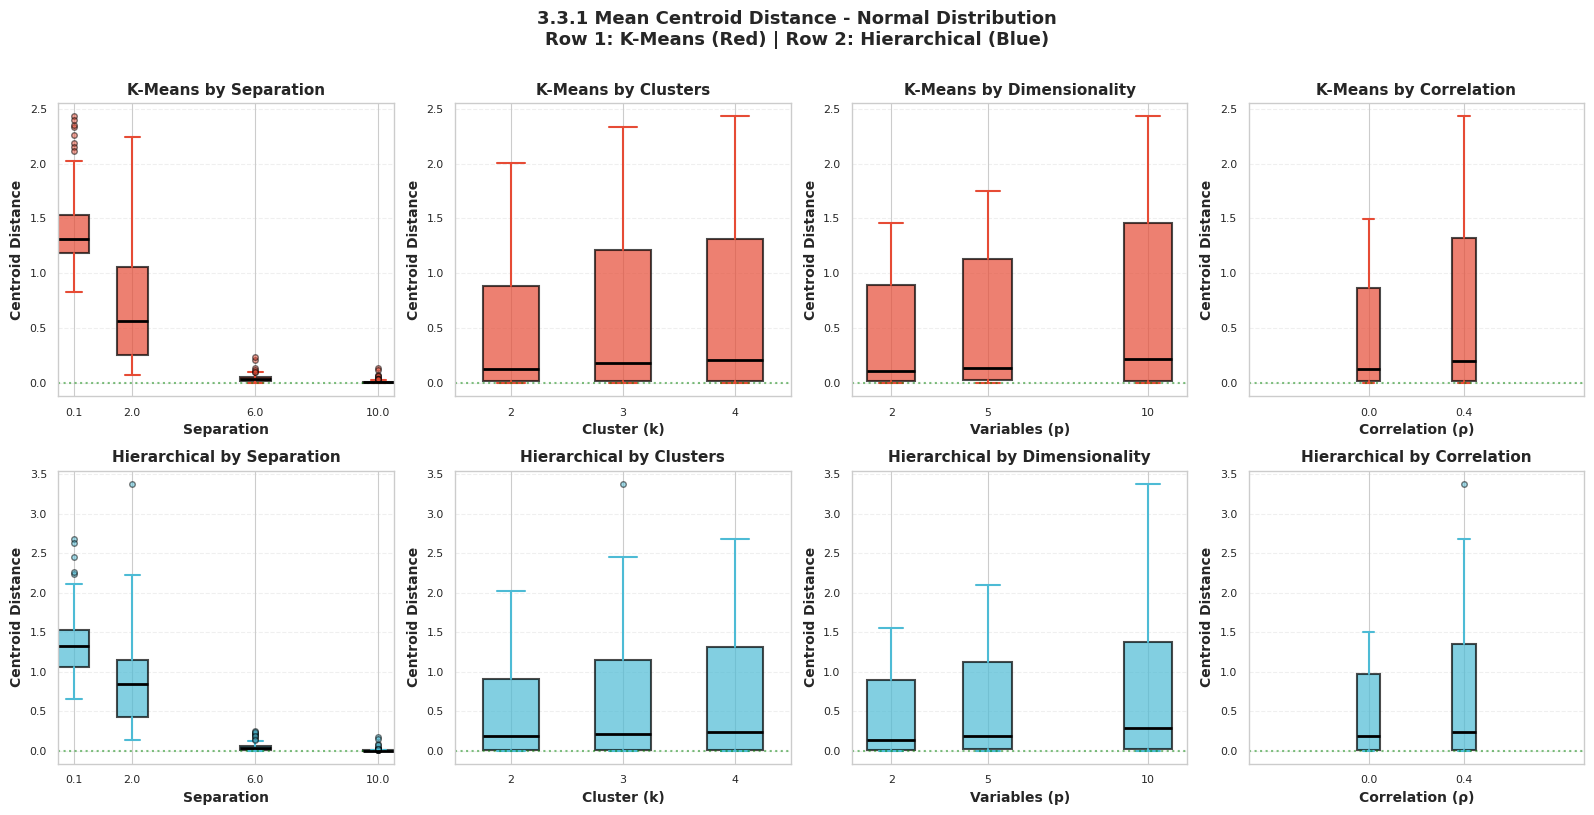
\includegraphics[width=\textwidth]{images/mcd_normal.png}
  \caption{\textbf{Mean Centroid Distance (Normal Distribution).} Row 1: K-Means. Row 2: Hierarchical Clustering.}
  \label{fig:mcd_normal}
  \source{Compiled by the author}
\end{figure}

\begin{figure}[H]
  \centering
  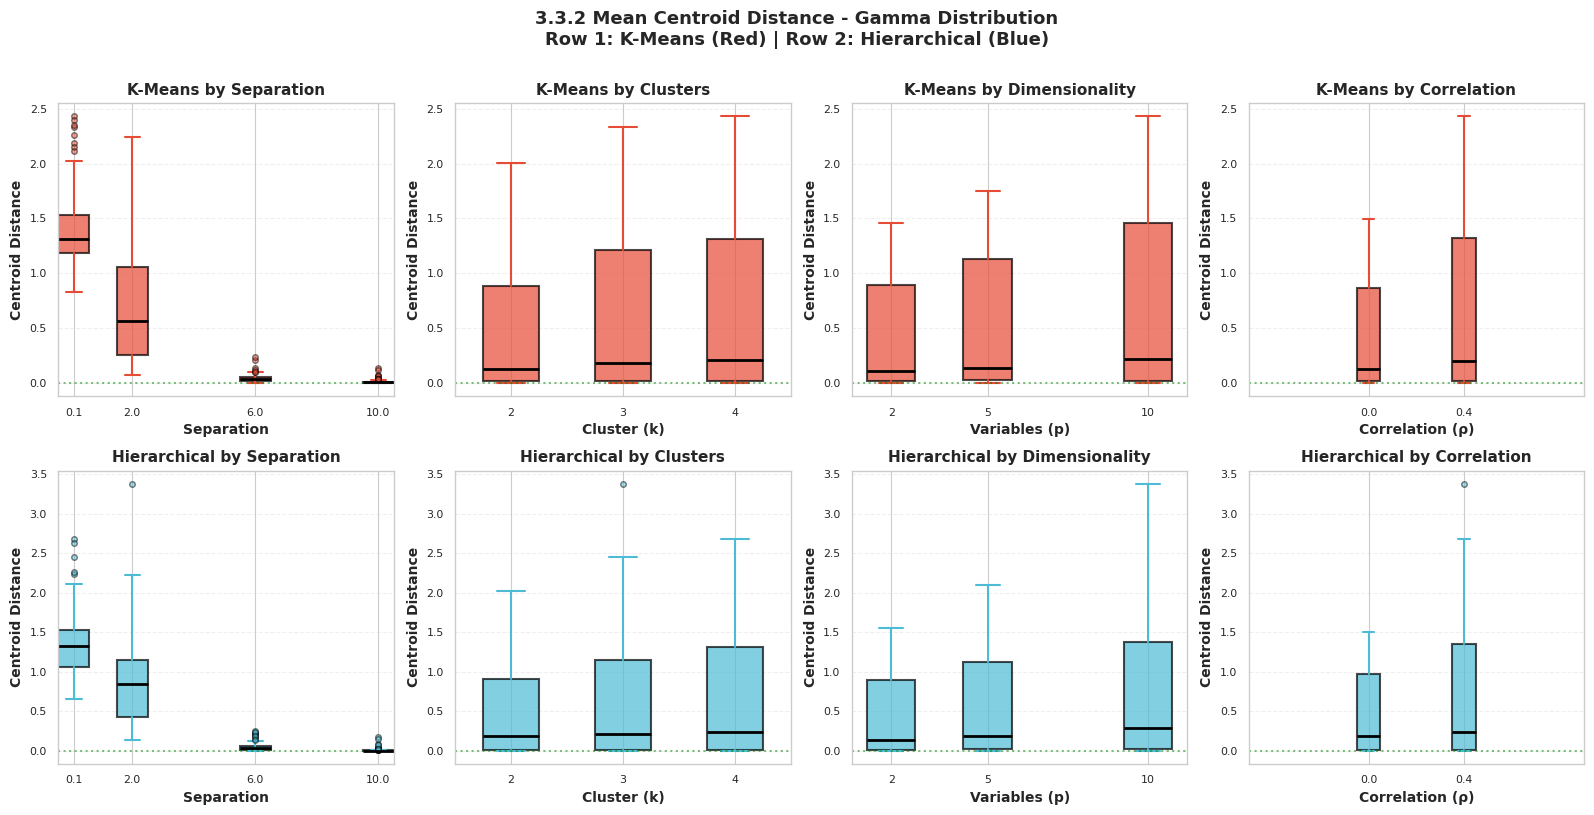
\includegraphics[width=\textwidth]{images/mcd_gamma.png}
  \caption{\textbf{Mean Centroid Distance (Gamma Distribution).} Row 1: K-Means. Row 2: Hierarchical Clustering.}
  \label{fig:mcd_gamma}
  \source{Compiled by the author}
\end{figure}

For both distributions, centroid drift is largest when cluster separation is low. As separation increases, the distance collapses toward zero. The main pattern is that complexity, especially high dimensionality and larger numbers of clusters, increases centroid instability. This indicates that synthetic generation struggles most when the structure is both sparse and high-dimensional.

\subsection{Mean Variance Difference}
\begin{figure}[H]
  \centering
  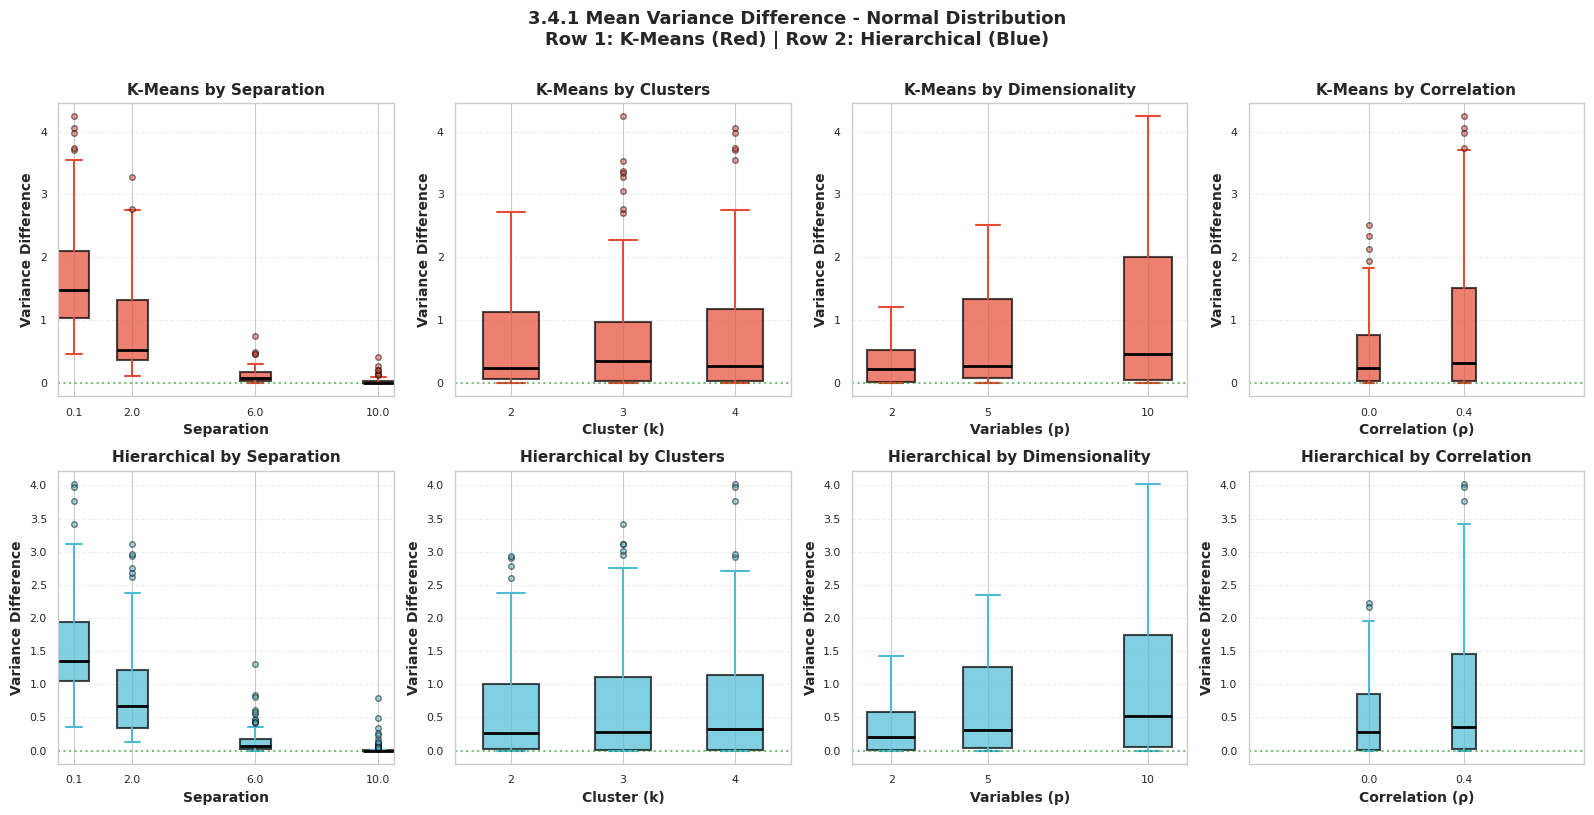
\includegraphics[width=\textwidth]{images/mvd_normal.png}
  \caption{\textbf{Mean Variance Difference (Normal Distribution).} Row 1: K-Means. Row 2: Hierarchical Clustering.}
  \label{fig:mvd_normal}
  \source{Compiled by the author}
\end{figure}

\begin{figure}[H]
  \centering
  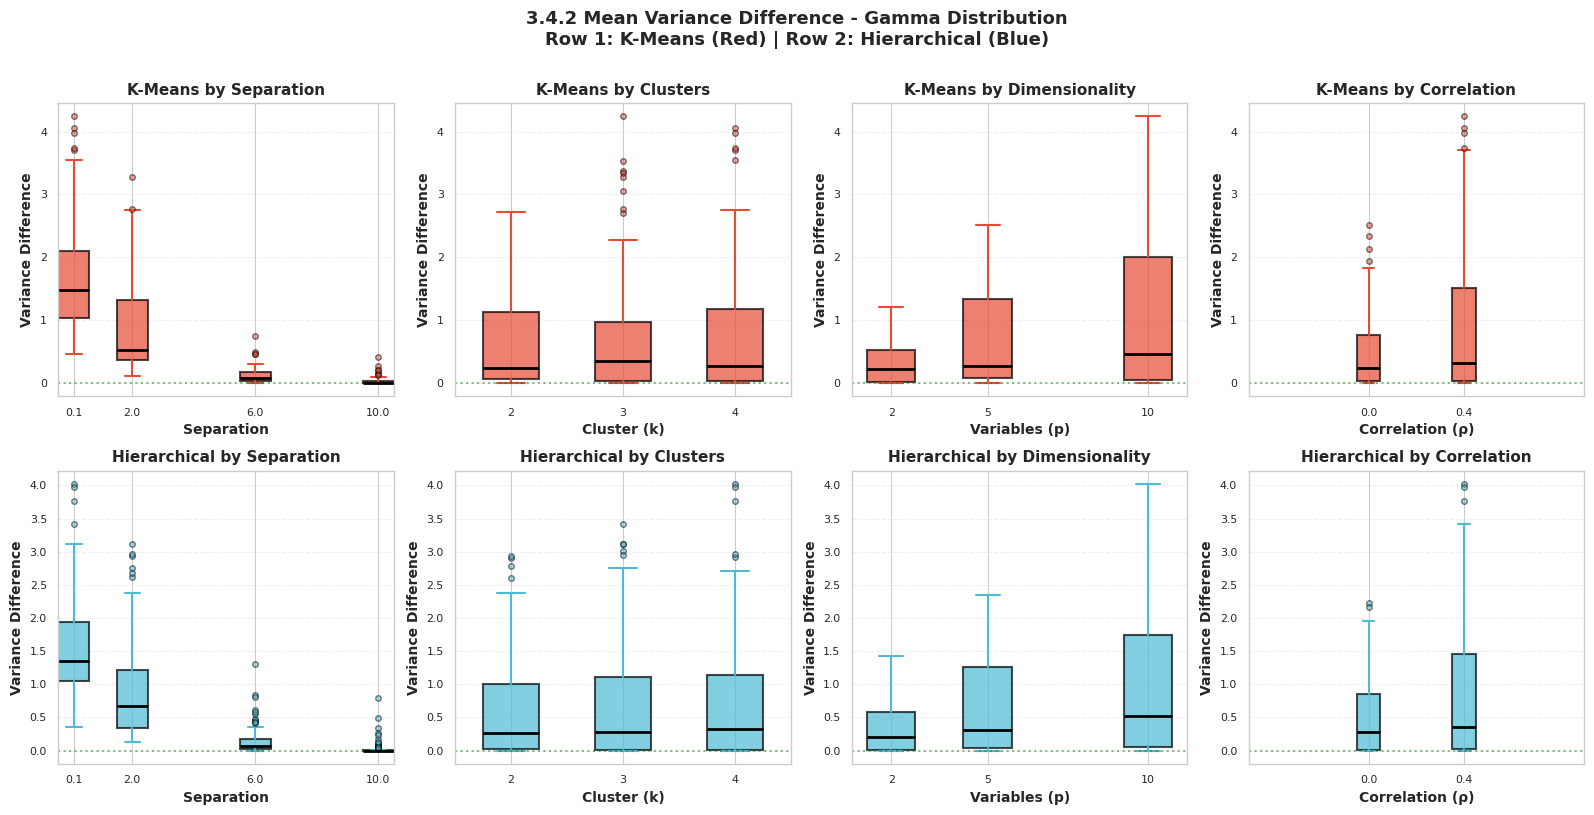
\includegraphics[width=\textwidth]{images/mvd_gamma.png}
  \caption{\textbf{Mean Variance Difference (Gamma Distribution).} Row 1: K-Means. Row 2: Hierarchical Clustering.}
  \label{fig:mvd_gamma}
  \source{Compiled by the author}
\end{figure}

Variance distortion follows a pattern similar to centroid drift. Low separation, higher dimensionality, and feature correlation make it difficult for the synthetic generator to preserve within-cluster compactness. This effect appears in both normal and gamma settings, which suggests that part of the distortion is intrinsic to the synthesis mechanism rather than to the specific distribution family.

\section{Evaluation Summary}
\label{sec:evaluation-summary}

The combined evidence supports a consistent interpretation:
\begin{itemize}
  \item synthetic data generated by CART is reliable for clustering when the original geometry is close to spherical and well separated;
  \item K-Means is highly sensitive to the blocky artifacts of synthesis in skewed settings;
  \item Hierarchical Clustering provides more robust cluster recovery and a more faithful representation of skewed structure;
  \item both algorithms experience meaningful degradation in high-dimensional, overlapping, or correlated conditions.
\end{itemize}
